\documentclass[12pt]{article}
\usepackage[UTF8]{ctex} % 加载中文支持宏包
\usepackage{amssymb}
\usepackage{amsmath}
\usepackage{graphicx}    % 如果需要插图
\usepackage{caption}
\usepackage{subcaption}  % 提供子图功能


\title{数论基础}
\author{ZZQ323}
% \date{}
\begin{document}
\maketitle

\tableofcontents

\begin{abstract}
    还在想的摘要hh
\end{abstract}
你好,LaTeX!

\section{小学的整数知识}


\begin{itemize}
    \item 整数可以表示成多项式 $n = c_{k}m^{k} + c_{k-1}m^{k-1} + c_{k-2}m^{k-2} +\dots+ c_{1}m^{1} + c_{0}m^{0}$ , 其中最高项不为0 $c_{k}\neq0$
    \item 如果b能整除a,那么b表示为 $b|a$,这个时候b是a的因数;r就是其中的余数。
    \item 素数(只能被……的自然数)、合数、整除、公因子、最大公因子gcd(或者用括号表示)、最小公倍数lcm
    \item 若$(a_{1},a_{2},a_{3},\dots,a_{n-1},a_{n})=1$,那么称 $a_{1},a_{2},a_{3},\dots,a_{n-1},a_{n}$ 互素;只有 $i,j \in [1,n] \&\&\;i\neq\;j\;\&\&\;(a_{i,a_{j}})=1$,这样才叫两两互素
    \item 整数之间的除法才有余数可言
    \item 因数分解最佳算法复杂度是$\ln^{\left(\dfrac{\ln n}{\ln\left(\ln n\right)}\right)^{\tfrac{1}{2}}}(n)$
    \item 为什么说最大的梅森素数是$M_{44497}=2^{44497}-1$?更大的就计算不出来了吗?
    \item 约定:a \%n 得到结果的正负由被除数a决定,与n无关
    \item 四则运算的结合律、交换律、分配律不影响取模
\end{itemize}

\section{带余除法}
\subsection{欧几里得算法}

首先根据带余除法这个式子,我们可以列出:
\begin{align}
    a &= bq_{1} + r_{1} \\
    b &= r_{1}q_{2} + r_{2} \\
    r_{1} &= r_{2}q_{3} + r_{3} \\
    \vdots\nonumber \\
    r_{n-3} &= r_{n-2}q_{n-1} + r_{n-1} \\
    r_{n-2} &= r_{n-1}q_{n} + r_{n}
\end{align}

首先$r_{1}<b$,否则的话多的部分会使得q变大来吸纳;
其次可以知道$b>r_{1}>r_{2}>\dots>r_{n-1}>r_{n}>0$;
这满足数列收敛的条件 —— 因此$r_{n}$有极限且极限为0;
由此一来,只要n足够大,那么最后一项就是:
\begin{equation}
    r_{n-2} = r_{n-1}q_{n}
\end{equation}
ps:有些参考书会写到n+1,其实都是一样的。

那么一步步反带入:

\begin{align}
    r_{n-2} &= r_{n-1}q_{n}\\
    r_{n-3} &= r_{n-2}q_{n-1}+r_{n-1}=r_{n-1}q_{n}q_{n-1}+r_{n-1}\\
    r_{n-4} &= r_{n-3}q_{n-2}+r_{n-2}=(r_{n-1}q_{n}q_{n-1}+r_{n-1})q_{n-2}+r_{n-1}q_{n}\\ \nonumber
            &=r_{n-1}q_{n}q_{n-1}q_{n-2}+r_{n-1}q_{n-2}+r_{n-1}q_{n}\\
    &\vdots\nonumber\\
    b &= g(q_{n},q_{n-1},q_{n-2},\dots,q_{4},q_{3})\cdot r_{n-1}\\
    r_{1} &= f(q_{n},q_{n-1},q_{n-2},\dots,q_{3},q_{2})\cdot r_{n-1}\\
    a &= h(q_{n},q_{n-1},q_{n-2},\dots,q_{2},q_{1})\cdot r_{n-1}
\end{align}

由于不同项数的组合顺序是不一样的,而且$q_{i}$之间也大概率不相同(偷懒);
所以不难看出:$f\neq g\neq h$(三个互不相等)。
进而证明了,a、b之间的gcd就是$r_{n-1}$。

\subsection{贝祖定理(Bézout's Identity) or 裴蜀定理}
如果$d = (a,b)$,则$\exists\;q、p\in Z \;,\;st.\;d=pa+qb$。
在算法中,我们可以理解为“有一系列的d,但是只有最小公倍数是这个式子里面最小的 —— 从而来化简式子”
证明如下:
因为存在$r_{n-1}$对a、b的唯一表示;
\begin{align}
    b &= g(q_{n},q_{n-1},q_{n-2},\dots,q_{4},q_{3})\cdot r_{n-1}\\
    a &= h(q_{n},q_{n-1},q_{n-2},\dots,q_{2},q_{1})\cdot r_{n-1}
\end{align}
所以,必然存在;
\begin{align}
    r_{n-1} &= \dfrac{b}{g(q_{n},q_{n-1},q_{n-2},\dots,q_{4},q_{3})}\\
    r_{n-1} &= \dfrac{a}{h(q_{n},q_{n-1},q_{n-2},\dots,q_{2},q_{1})}
\end{align}
也就是
\begin{align}
    gcd(a,b) &= d = \dfrac{b}{g(q_{n},q_{n-1},q_{n-2},\dots,q_{4},q_{3})}\\
    gcd(a,b) &= d = \dfrac{a}{h(q_{n},q_{n-1},q_{n-2},\dots,q_{2},q_{1})}
\end{align}
但是还是不够明确,回到之前的:
\begin{align}
    r_{n-2} &= r_{n-1}q_{n}\\
    r_{n-3} &= r_{n-2}q_{n-1}+r_{n-1}=r_{n-1}q_{n}q_{n-1}+r_{n-1}\\
    r_{n-4} &= r_{n-3}q_{n-2}+r_{n-2}=(r_{n-1}q_{n}q_{n-1}+r_{n-1})q_{n-2}+r_{n-1}q_{n}\\ \nonumber
            &=r_{n-1}q_{n}q_{n-1}q_{n-2}+r_{n-1}q_{n-2}+r_{n-1}q_{n}\\
    \vdots\nonumber\\
    b &= g(q_{n},q_{n-1},q_{n-2},\dots,q_{4},q_{3})\cdot r_{n-1}\\
    r_{1} &= f(q_{n},q_{n-1},q_{n-2},\dots,q_{3},q_{2})\cdot r_{n-1}\\
    a &= h(q_{n},q_{n-1},q_{n-2},\dots,q_{2},q_{1})\cdot r_{n-1}\\
    a &=bq_{1}+r_{1}
\end{align}

然后带入到最初的式子:
\begin{align}
    a&=bq_{1}+r_{1}\\
    a&=bq_{1}+f(q_{n},q_{n-1},q_{n-2},\dots,q_{3},q_{2})\cdot r_{n-1}\\
    r_{n-1}&=\frac{1}{f(q_{n},q_{n-1},q_{n-2},\dots,q_{3},q_{2})}a+\frac{q_{1}}{f(q_{n},q_{n-1},q_{n-2},\dots,q_{3},q_{2})}b
\end{align}

然后 …… 好像也没证明

正确的证明是:

\begin{align}
    a &= bq_{1} + r_{1} \\
    r_{1} &= a - bq_{1} \\
    b &= r_{1}q_{2} + r_{2} \\ \nonumber &= (a - bq_{1})q_{2} + r_{2} \\
    r_{2} &= b - (a - bq_{1})q_{2}\\
    r_{1} &= r_{2}q_{3} + r_{3} \\ \nonumber &= (b - (a - bq_{1})q_{2})q_{3} + r_{3}\\
    \vdots\nonumber \\
    r_{n-1}&=F(q)a+G(q)b
\end{align}

\section{GCD相关的知识}
\subsection{奇奇怪怪的等式}
\begin{align}
    gcd(a,b) &=gcd(a,a+b)\nonumber \\
    &=gcd(a,k\cdot a+b)\nonumber  \\ 
    &=gcd(a+k\cdot b,b)\nonumber
\end{align}

由贝祖定理知:如果$d = (a,b)$,则$\exists\;q、p\in Z \;,\;st.\;d=pa+qb$。
而上面两个式子无非就是令$b=ka+b$或者$a=kb+a$,展开来都是一致的,不需要证明什么东西。
甚至,你令$a=\dfrac{a+b}{2}$、$b=\dfrac{a-b}{2}$,这样搞换底也是可以的。


\subsection{拉梅定理}
用欧几里得算法计算两个正整数的最大公约数,需要的除法次数不会超过两个整数中
较小的那个十进制数的位数的5倍。

其实也就是:$O(n)\leq 5\log_{10}(\min (a,b))$

\subsection{欧几里得算法、更相减损数、Stein算法}

不知道怎么插入代码

\subsection{LCM}

\subsection{代数基本定理}
任意一个大于1的正整数都可以被分解为素数的乘积;
\begin{displaymath}
    n=P_{1}^{\alpha_{1}} P_{2}^{\alpha_{2}} P_{3}^{\alpha_{3}} P_{4}^{\alpha_{4}} P_{5}^{\alpha_{5}}
\end{displaymath}

\subsection{计算方法证明}
下面假设:
\begin{align}
    a&=p_{1}^{c_{1}} p_{2}^{c_{2}} \cdots p_{n}^{c_{n}}\\
    b&=p_{1}^{f_{1}} p_{2}^{f_{2}} \cdots p_{n}^{f_{n}}
\end{align}
所以:
\begin{align}
    gcd(a,b) &= p_{1}^{c_{1}} p_{2}^{c_{2}} \cdots p_{n}^{c_{n}} \cdot p_{1}^{f_{1}} p_{2}^{f_{2}} \cdots p_{n}^{f_{n}} \\
    &=p_{1}^{\min (c_{1},f_{1})} p_{2}^{\min (c_{2},f_{2})} \cdots p_{n}^{\min (c_{n},f_{n})}\\
    lcm(a,b) &= p_{1}^{\max (c_{1},f_{1})} p_{2}^{\max (c_{2},f_{2})} \cdots p_{n}^{\max (c_{n},f_{n})}\\
    gcd(a,b)\cdot &lcm(a,b) = a\cdot b
\end{align}


\subsection{LCM与GCD的关系}

观察例题 \ref{fig.lcm-gcd-relation}:

\begin{figure}[!htb]
    \centering
    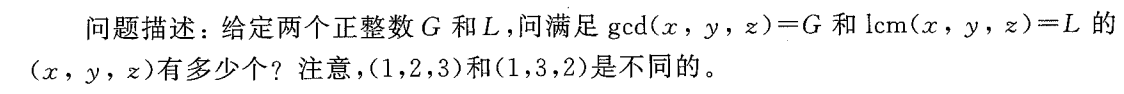
\includegraphics[width=\textwidth]{./images/hdu4497}
    \caption{一道hdu4497的例题}
    \label{fig.lcm-gcd-relation}
\end{figure}

这里有一个显然的性质:
\begin{displaymath}
    L \% G \equiv 0
\end{displaymath}



\section{丢番图}
在学习丢番图方程时,常从线性或简单二次形式入门,再逐步了解更复杂的高次或几何形式。

主要有以下类型:
\begin{itemize}
    \item 线性丢番图:$ax+by=c$
    \item 多元线性丢番图:$a_{1}x_{1}+a_{2}x_{2}+a_{3}x_{3}+\cdots+a_{n-1}x_{n-1}+a_{n}x_{n}=c$
    \item 高次丢番图:$x^{n}+y^{n}=z^{n}$
    \begin{itemize}
        \item 勾股定理:$x^{2}+y^{2}=c^{2}$
        \item 大费马定理:$x^{n}+y^{n}=z^{n}\quad $when $n>2$ the equation is invalid.
        \item Pell方程(一个双曲线):$x^{2}-Dy^{2}=1$
    \end{itemize}
    \item 指数丢番图:$a^{x}+b^{y}=c^{z}$
\end{itemize}

相关问题:
椭圆方程上的有理点构造问题。
扩展欧几里得算法(线性情况)、连分数法(二次Pell方程)、Lattice-based 方法(格上求解)。

\section{二阶丢番图解的通解问题}

\subsection{图解证明}

对于$ax + by = c$,如果\(\gcd(a,b) \mid c\) (也就是$c \% \gcd(a,b) = 0$)

注:这里的c也可能是的负的 …… 因为 …… 

对于一个特解$x_{0}$、$y_{0}$,我可以很顺利地得到对应的整数通解:
\begin{align*}
    x&=x_{0}+\frac{b}{\gcd(a,b)}n\\
    y&=y_{0}-\frac{a}{\gcd(a,b)}n
\end{align*}
原因就是:x每增加一个1 $x=x_{0}+n$ ,那么对应到等式中y就需要减少一个$\frac{a}{b}$

那么x每增加一个b $x=x_{0}+bn$,那么对应到等式中y就需要减少一个$\frac{ab}{b}=a$

基于此,给x和y的系数同时除以$\gcd$,那么就可以得到\textbf{最小步长的通解公式},保障不会漏掉什么通解。

% 其实还可以这么想:$ax + by = a(\frac{c}{d}x_{0}) + b(\frac{c}{d}y_{0}) = c$

但要是如果\(\gcd(a,b) \nmid c\) (也就是$c \% \gcd(a,b) \neq 0$),那么就不会有任何一个点在格子点上,自然也不会有什么整数解 …… 一个解都没有!

\begin{figure}[htb!]
    \centering
    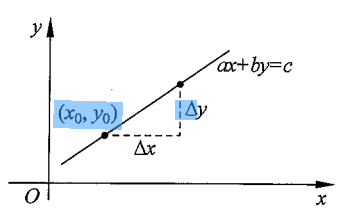
\includegraphics[width=0.5\textwidth]{./images/二阶丢番图.png}
    \caption{二阶丢番图图解}
    \label{fig.sth}
\end{figure}

\subsection{扩展欧几里得算法求特解}

首先已知:$pa+qb=\gcd(a,b)$;
这里只是把$pa+qb=\gcd(a,b)$写成了$xa+yb=\gcd(a,b)$;
由前面的步骤可知,x、y都是$f(q)$,只要从上往下化简,表示出$r_{n-1}$,其中的一大坨$q_{n}$就是x以及y了;

但是具体的:

\begin{align}
    a &= bq_{1} + r_{1} \\
    r_{1} &= a - bq_{1} \\
    b &= r_{1}q_{2} + r_{2} \\ \nonumber &= (a - bq_{1})q_{2} + r_{2} \\
    r_{2} &= b - (a - bq_{1})q_{2}\\
    r_{1} &= r_{2}q_{3} + r_{3} \\ \nonumber &= (b - (a - bq_{1})q_{2})q_{3} + r_{3}\\
    \vdots\nonumber \\
    r_{n-1}&=F(q)a+G(q)b
\end{align}

在这里我们改写成:$r_{n-1}=xa+yb$,也即:

\begin{align*}
    x&=F(q)\\
    y&=G(q)
\end{align*}

怎么计算这么长的F、G呢?

注意到,在最小一个子问题的讨论中,我们会得到$a^{'}x+b^{'}y=\gcd(a,b)$。

那么,在上一层的求解中,我们就知道了下一层已经满足了这个条件;
但是,我们保存了每一层的a、b,子递归中的a、b并非我们所有的a、b,所以我们需要调整x、y以适应这一层a、b的结论

\begin{align*}
    &\begin{cases}
        a' = b,\\
        b' = a \mod b,
    \end{cases}\\
    &\Rightarrow bx+(a\mod b)y=gcd(a,a\mod b)=gcd(a,b)\\
    &\Rightarrow bx+(a\mod b)y=bx+(a-\lfloor\frac{a}{b}\rfloor*b)y=gcd(a,b)\\
    &\Rightarrow ay+bx-\lfloor\frac{a}{b}\rfloor*b y=gcd(a,b)\\
    &\Rightarrow ay+b(x-\lfloor\frac{a}{b}\rfloor y)=gcd(a,b)
\end{align*}

那么对于这一层的x、y,是不是又能通过下面那一层的x、y模拟了呢?
\begin{align*}
    y&=x_{\text{下}}-y_{\text{下}}\\
    x&=y_{\text{下}}
\end{align*}



\subsection{丢番图例题*可跳过}

主要是算法问题
\begin{figure}[htb!]
    \centering
    \begin{subfigure}{1\textwidth}
        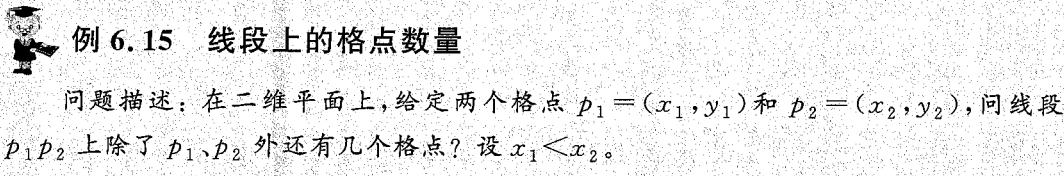
\includegraphics[width=\textwidth]{./images/6.15}
        \caption{题目\ref{fig.exa_1}}
        \label{fig.exa_1}
    \end{subfigure}
    \begin{subfigure}{1\textwidth}
        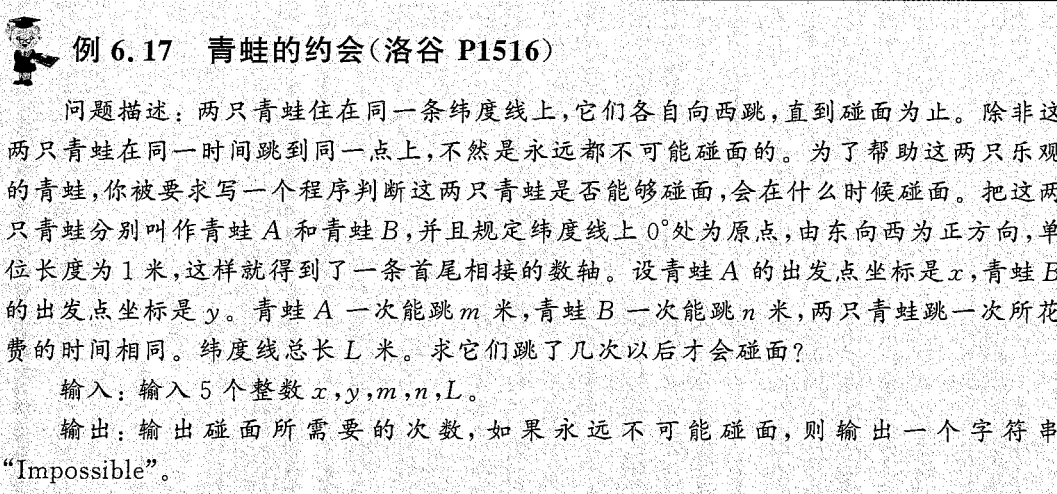
\includegraphics[width=\textwidth]{./images/6.17}
        \caption{题目\ref{fig.exa_2}}
        \label{fig.exa_2}
    \end{subfigure}
    \caption{}
    \label{fig.exa}
\end{figure}

顺便复习c++饿啊啊啊。

\subsection{多元丢番图}

实际上就是形如:$a_{1}x_{1}+a_{2}x_{2}+a_{3}x_{3}+\cdots+a_{n-1}x_{n-1}+a_{n}x_{n}=c$ 式子的这么一个解。

当且仅当$\gcd(a_{1},a_{2},a_{3},\cdots,a_{n-1},a_{n}) \mid c$,这个方程组有tmd无数个解。

然后呢,像下面这样直接求解就行了。


\begin{displaymath}
    \left\{
        \begin{aligned}
            &a_{1}x_{1}+a_{2}x=d_2t_2\\
            &d_{2}t_{2}+a_{2}x=d_3t_3\\
            &\vdots\\
            &d_{n-1}t_{n-1}+a_{n}x=d_nt_n
        \end{aligned}
    \right.
\end{displaymath}


\section{同余}
长成:$a\equiv b(\mod n)$ 就是同余式。

\subsection{基本性质}

\begin{enumerate}
    \item 正整数a,b对n取模,它们的余数相同,记作:$a\equiv b(\mod n)$
    \item 若$a-k*n=b$,则$a\equiv b(\mod n)$;换而言之,我们可以将同余式 $a\equiv b(\mod n)$ 与等式 $a\equiv b+k*n$ 互化
    \item 若$a\equiv b(\mod n)$且$c\equiv b(\mod n)$,则$a\equiv c(\mod n)$
    \item 若$a\equiv b(\mod n)$,则$a+c\equiv b+c(\mod n)$ 
    \item 若$a\equiv b(\mod n)$,且$c\equiv d(\mod n)$,则 $a+c\equiv b+d(\mod n)$ or $a+d\equiv b+c(\mod n)$(乘法的结论类似)
\end{enumerate}


\subsection{一元线性同余方程}

若$a-k*m=b$,则$a\equiv b(\mod m)$;换而言之,我们可以将同余式 $a\equiv b(\mod m)$ 与等式 $a\equiv b+k*m$ 互化.

那么,基于此$ax\equiv b(\mod m) \quad \Rightarrow \quad ax+my=b$;

设$d=\gcd(a,m)$,如果有$d \mid b$(也即$b\mod d == 0$),那么有d个解答;反之无解。

至于为什么有d个,那是因为:$x=x_{0}+\frac{m}{d}n$,由于解之间的间隔是 $\frac{m}{d}$,模 
m 下的解是周期性的,而每个解对应于不同的同余类。


\subsection{费马小定理}

\subsubsection{二项式式展开证明}
考虑$(1+x)^{p}$的二项式展开:
\begin{align*}
    (1+x)^{p} = \sum_{i=0}^{p}\binom{p}{i}a_{i} = \binom{p}{0}a_{0} + \binom{p}{1}a_{1} + \binom{p}{2}a_{2} + \dots + \binom{p}{p-1}a_{p-1} + \binom{p}{p}a_{p}
\end{align*}

根据:$C_{n}^m=\dfrac{n!}{(n-m)!m!}$,且p是素数的情况下,我们知道:除了$C_{p}^{0}$ 或 $C_{p}^{p}$,其他都会被mod p 给化掉:

\begin{align*}
    (1+x)^{p} &= \binom{p}{0}a_{0} + \binom{p}{p}a_{p} = 1+x^{p} (\mod p)\\ 
    (1+x)^{p} &- x^{p} = 1 (\mod p)
\end{align*}

这就是经典的幂函数数列$b_{n}=n^{p}$,上述式子可化为:$b_{n+1}-b_{n}=1$。
由累加可得:$b_{n}=b_{1}+n-1=1^{p}+n-1=n$,则$b_{a}=a^{p}=a$

德政

\subsubsection{多项式展开证明}
考虑$a^{p}$的多项式展开:
\begin{align*}
    (1_{1}+1_{2}+1_{3}+\dots+1_{a-1}+1_{n})^{p}&=\sum_{i=0}^p\binom{p}{k_{1},k_{2},\dots,k_{n}}1^{x}=\sum_{i=0}^p\binom{p}{k_{1},k_{2},\dots,k_{n}}
\end{align*}

在$\mod p$且$p$是质数的情况下,除了$\binom{p}{p,0,0,\dots,0,0}$、$\binom{p}{0,p,0,\dots,0,0}$等等都会变成0(因为没有数能消掉p除了它自己);

ps:$\binom{n}{n_{1},n_{2},n_{3},\dots,n_{m-1},n_{m}}=\dfrac{n!}{n_{1}!n_{2}!\dots n_{m-1}!n_{m}!}$

那么在全选一个的情况下,就会有:

\begin{align*}
    (1_{1}+1_{2}+1_{3}+\dots+1_{a-1}+1_{n})^{p}=a^{p}=1^{p}+1^{p}+\dots+1^{p}+1^{p}=a(\mod p)
\end{align*}

德政

\subsubsection{模算法证明*}

我们首先考虑整数$a,2a,3a,\dots ,(p - 1)a$。这些数都不等于p对其他数的模,也不等于0。
如果这样,那么有:$r × a \equiv s × a (\mod p),1 \leq r < s \leq p - 1$;
那么,两边消去a将得到 $r\equiv (mod p)$,这是不可能的,因为r和s都在1和p - 1之间。

因此,前一组整数想要同余到$1,2,\dots p - 1$。必须把这些同余相乘,你会发现:
$a × 2a × 3a × ... × (p - 1) × a \equiv 1 × 2 × 3 × ... × (p - 1)(mod p)$
意味着:
$a^{p-1} × (p - 1)! \equiv (p - 1)!(mod p)$。
从这个表达式的两边消去$(p - 1)!$,我们得到:
$a^{p-1} \equiv 1 (mod p)$。


\section{欧拉定理}




\section{求逆}


\end{document}
